\chapter{Materiales y Productos}
\section{Introducción.}
\subsection{Clasificación global.}
Los materiales más empleados en construcción son: acero, hormigón, áridos, fábrica y mezclas bituminosas y asfaltos. Otros materiales frecuentes son: madera, aluminio, vidrio, plásticos, materiales compuestos, etc. Y por supuesto el suelo como estructura.

\subsection{Evolución en la ciencia de materiales.}
Hoy en día la ciencia de materiales evoluciona a gran velocidad existiendo numerosos materiales que empiezan a ser competencia real de los tradicionales, entre ellos:
\begin{itemize}
    \item Polímeros, adehivos, materiales compuestos, geotextiles, recubrimientos, metales conformados en frío, productos sintéticos, etc.
\end{itemize}
Además proliferan nuevos aditivos que modifican a conveniencia las características de los materiales base, especialmente en los hormigones, elastómeros y asfaltos.
\begin{itemize}
    \item Características mecánicas: resistencia, ductilidad, dureza, maleabilidad, etc.
    \item Comportamiento frente a corrosión, magnetismo, temperatura, etc.
    \item Características estéticas: acabados, texturas, color, etc.
\end{itemize}
Un último punto a tener en cuenta es la necesidad de emplear y/o generar materiales reciclados y/o reciclables.

\subsection{Propuedades mecánicas.}
Caracterizan la respuesta del material ante acciones externas:
\begin{itemize}
    \item Resistencia: Variable en función del tipo de fuerza, la edad del material, el contenido de humedad, la temperatura, \dots
    \item Resistencia a la deformación: Dependiente de la rigidez, ductilidad, edad, temperatura, \dots
    \item Dureza: Resistencia al corte de la superficie, abrasión, desgaste.
    \item Resistencia a la fatiga: Pérdida de resistencia con el tiempo ante acciones repetidas.
\end{itemize}

\subsubsection{Ley de comportamiento del material.}
Representa la curva $\sigma - \epsilon$ obtnida en un ensayo de caracterización del material. Cada material responde de manera diferente ante el efecto de una carga, ejemplo típicos de comportamiento diferentes son:

\begin{figure}[H]
    \centering
    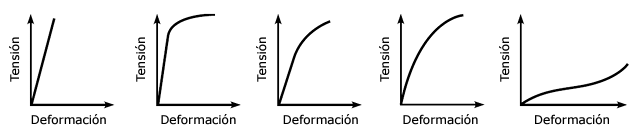
\includegraphics[width = 0.5 \textwidth]{Imagenes/Ley de comportamiento del material.png}
\end{figure}

\begin{table}[H]
    \centering
    \begin{tabular}{| l | p{2cm} | p{2cm} |}
        \hline
        \rowcolor{lightgray} Material & Módulo de Young (GPA) & Coeficiente de Poisson \\
        \hline
        Acero & 207 & 0.27 \\
        Fundición de hierro & 75 - 169 & 0.17 \\
        Cobre & 110 & 0.35 \\
        Aluminio & 69 - 75 & 0.35 \\
        Hormigón & 14 - 40 & 0.11 - 0.21 \\
        Ladrillo & 10 - 17 & 0.23 - 0.40 \\
        Roca Caliza & 58 & \\
        Vidrio & 62 - 70 & 0.25 \\
        Madera & 6 - 15 & \\
        Epoxy & 3 - 140 & \\
        Goma (blanda) & 0.001 - 0.014 & 0.49 \\
        \hline
    \end{tabular}
\end{table}

\begin{figure}[H]
    \centering
    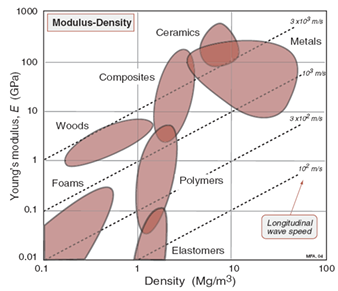
\includegraphics[width = 0.5 \textwidth]{Imagenes/Grafica Modulo de Young - Densidad.png}
\end{figure}

\subsubsection{Propiedades no mecánicas.}
No influyen en la ley de comportamiento del material
\begin{itemize}
    \item Densidad: Propiedad física que influye en la solicitación que debe resistir la estructura
    \item Propiedades térmicas: Conductividad, calor específico, punto de fusión, coeficiente de expansión térmica. Algunas de estas propiedades influyen en la resistencia al fuego del material.
    \item Durabilidad: Resistencia al clima, corrosión, desgaste, \dots
    \item Propiedades eléctricas y magnéticas: Resistividad, constante dieléctrica, permeabilidad magnética, \dots
    \item Trabajabilidad: Moldeado, ensamblaje, modificación, \dots
    \item Estética
    \item Disponibilidad y coste
\end{itemize}


\section{Hormigón.}
Mateiral formado por cemento, áridos y agua, y a veces, aditivos (inciden favorablemente en las propiedades del hormigón).

\begin{itemize}
    \item Cemento. $Calizas\ +\ Arcillas\ \rightarrow\ Pulverizacion\ mezcla\ calcinacion\ \rightarrow\ Clinker$. $Cliker\ +\ Yeso\  \rightarrow\ Pulverizacion\ \rightarrow\ Cemento$.
    \item Áridos. Arenas, gravas, rocas machacadas, escoria siderúrgica. Pueden ser áridos finos o arenas ($\phi \leq 4 mm$) y áridos gruesos o gravas ($\phi > 4mm$). La superficie total de los áridos ha der ser la menor posible en relación a su volumen: Dosificación adecuada.
    \item Agua. En general, cualquier agua es aceptable, excepto la del mar (por su alto contenido en cloruros), la de la montaña (por su agresividad) y las aguas pantanosas (por la existencia de limos, algas y residuos que dificultan la adherencia pasta-árido).
\end{itemize}

\subsection{Características tecnológicas.}
Estas propiedades son las que nos indican la disposición de un material para poder trabajar con él o sobre él.

\subsubsection{Docilidad.}
Capacidad de la masa de rellenar el molde sin dejar huecos con los procedimientos de compacación previstos en obra. Se mide mediante el asiento del cono de abrams (figura \ref{fig: Cono de Abrams}).
\begin{table}[H]
    \centering
    \begin{tabular}{c c}
        Tipo de consistencia & Asentamiento en cm \\
        \hline
        Seca (S) & 0 - 2 \\
        Plástica (P) & 3 - 5 \\
        Blanda (B) & 6 - 9 \\
        Fluida (F) & 10 - 15 \\
        Liquida (L) & 16 - 20 \\
    \end{tabular}
\end{table}
Salvo en aplicaciones especificas que así lo requieran, se evitará el empleo de las consistencias seca y plástica. No podrá emplearse la consistencia líquida, salvo que se consiga mediante el empleo de aditivos superplastificantes.

\begin{figure}[H]
    \centering
    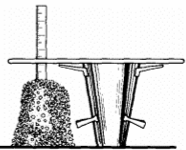
\includegraphics[width = 0.25 \textwidth]{Imagenes/Cono de Abrams.png}
    \label{fig: Cono de Abrams}
    \caption{Cono de Abrams}
\end{figure}

Cono de Abrams: Molde troncocónico de 30 cm de altura que se rellena del hormigón a ensayar y se voltea. Se mide lo que asienta la masa del hormigón.

\subsubsection{Homogeneidad.}
Es la propiedad por la cual los diferentes componentes del hormigón aparecen regularmente distribuidos entoda la masa, de manera tal que dos muestras tomadas de distintos lugares de la misma resulten prácticamente iguales. La homogeneidad s econsigue con un buen amasado y, para mantenerse, requiere un transporte cuidadoso y una colocación adecuada.

La homogeneidad puede perderse por segregación (separación de los gruesos por una parte y los finos por otra) o por decantación (los granos gruesos caen al fondo y el mortero queda en la superficie, cuando la mezcla es muy líquida).

Ambos fenómenos aumentan con el contenido de agua, con el tamaño máximo del árido, con las cibraciones o sacudidas durante el transporte y con la puesta en obra en caída libre.

\subsection{Características reológicas.}
Estas propiedades son las que permiten caracterizar el comportamiento del material a lo largo del tiempo.

\subsubsection{Fluencia.}
Es la deformación que sufre el hormigón a lo largo del tiempo sin que se produzca un incremento en las cargas aplicadas.
\[ \epsilon_{C \sigma} (t, t_0) = \sigma (t_0) \cdot \left( \frac{1}{E_{0, t_0}} + \frac{\phi(t, t_0)}{E_{0,28}} \right) \]
\[ \phi(t, t_0) = \phi_0 \cdot \beta_c (t - t_0) \]

Siendo:
\begin{itemize}
    \item $t_0$: Edad del hormigón (puesta en carga)
    \item $E_{0, t_0}$: Deformación isntantánea
    \item $E_{0, 28}$: Deformación diferida
    \item $\phi_0$: Coeficiente básico de fluencia instantáneas
    \item $\beta_c$: Desarrollo en el tiempo
\end{itemize}

\begin{figure}[H]
    \centering
    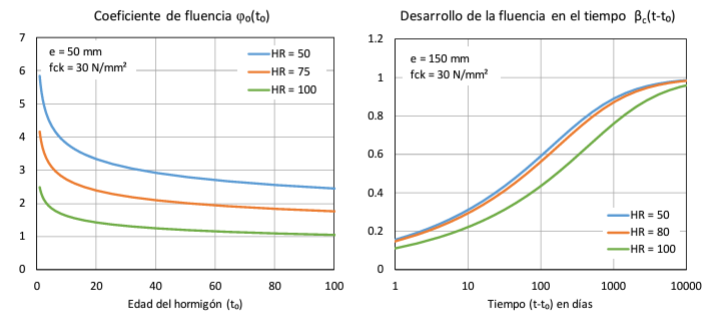
\includegraphics[width = 0.5 \textwidth]{Imagenes/Graficas Fluencia.png}
\end{figure}

\subsubsection{Retracción.}
Es la deformación que sufre el hormión a lo largo del tiempo como consecuencia del gradiente de humedades entre el material y el medio ambiente. A la contracción del hormigón como consecuencia de la pérdida de agua se opone la armadura originándose uan fisuración superficial y tensiones remanentes internas. Depende de la humedad relativa, dosificación y grenulometría del hormigón, diámetros de las armaduras y distribución, dimensiones de la pieza,... 

Tipos de retracción:
\begin{itemize}
    \item Por consolidación y segregación.
    \item Plástica: Se produce en el fraguado cuando la velocidad de evaporación del agua supera a la de exudación.
    \item Hidráulica: Se produce después del curado.
\end{itemize}

\subsubsection{Cansancio.}
Es la disminución de la capacidad resistente del hormigón como consecuencia de la aplicación de cargas lentas en comparación al valor que se obtiene ante cargas rápidas.

\begin{figure}[H]
    \centering
    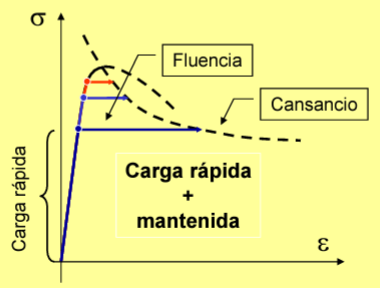
\includegraphics[width = 0.25 \textwidth]{Imagenes/Curva Cansancio.png}
\end{figure}

\subsection{Características mecánicas.}

\begin{figure}[H]
    \centering
    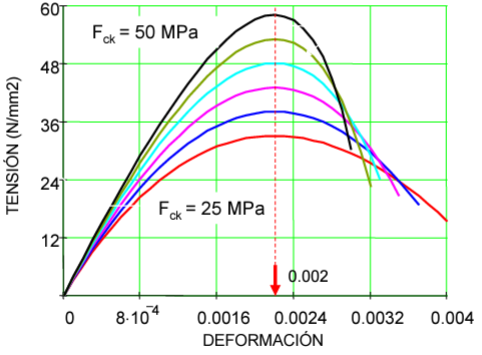
\includegraphics[width = 0.5 \textwidth]{Imagenes/Comportamiento a compresion para cargas instantaneas.png}
    \caption{Comportamiento a compresión para cargas instantáneas.}
\end{figure}

% Comportamiento a compresión hormigón

\begin{figure}[H]
    \centering
    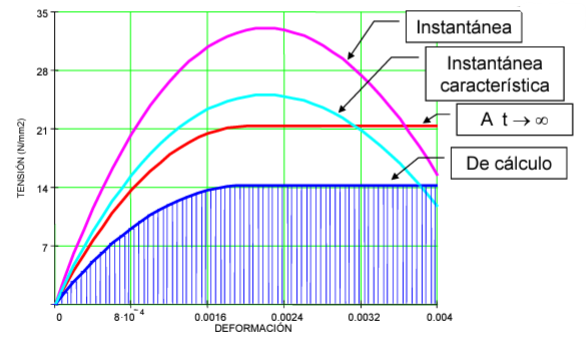
\includegraphics[width = 0.5 \textwidth]{Imagenes/Comportamiento a compresion hormigon.png}
    \caption{Comportamiento a compresión hormigón.}
\end{figure}

% Propiedades de cálculo para hormigón armado

\begin{figure}[H]
    \centering
    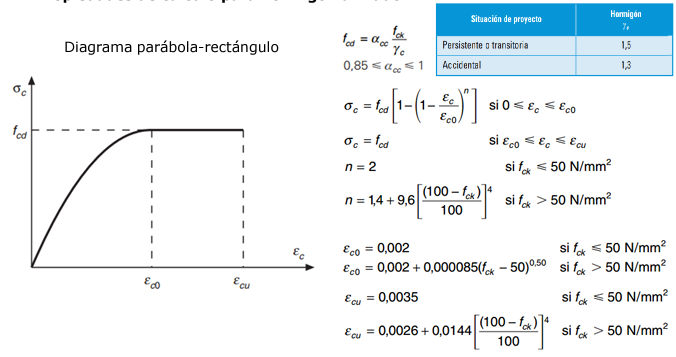
\includegraphics[width = 0.5 \textwidth]{Imagenes/Propiedades de calculo para hormigon armado.png}
    \caption{Propiedades de cálculo para hormigón armado.}
\end{figure}

\subsubsection{Resistencia a tracción.}
Normalmente se refiere a la resistencia característica. Las expresiones más usadas son:
\begin{itemize}
    \item Característico: $f_{ct, k} = 0,21 \cdot \sqrt[3]{f_{ck}^2}$
    \item Medio: $f_{ct, m} = 0,30 \cdot \sqrt[3]{f_{ck}^2}$
    \item Cuantil $95\%$: $f_{ct, k 0,95} = 0,39 \cdot \sqrt[3]{f_{ck}^2}$
\end{itemize}
Escasa aplicación en proyecto.

\subsubsection{Rigidez.}
Al no ser el hormigón un cuerpo  elástico, más que hablar de módulo de elasticidad habría que hablar de módulo de deformación longitudinal, el cual no es constante. Se distinguen los siguientes parámetros:
\begin{itemize}
    \item Módulo tangente ($E_{c, tang}$): Mide la inclinación de la tangente a la curva.
    \item Módulo secante ($E_{c, sec}$): Mide la inclinación de la recta que une el origen con cada punto de la curva.
    \item Módulo inicial ($E_{c,0}$): Inclinación de la tangente a la curva en el origen.
    \item Módulo instantáneo ($E_{c, sec45}$): Es la pendiente de la secante cuando se alcanza el $45 \%$ de la resistencia característica compresiva.
\end{itemize}

\begin{figure}[H]
    \centering
    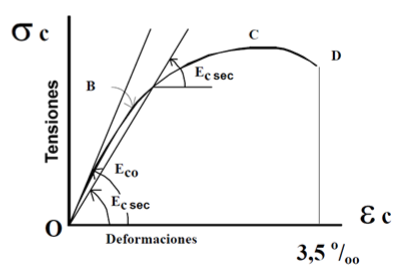
\includegraphics[width = 0.5 \textwidth]{Imagenes/Rigidez.png}
\end{figure}

\subsection{Especificación.}

\begin{figure}[H]
    \centering
    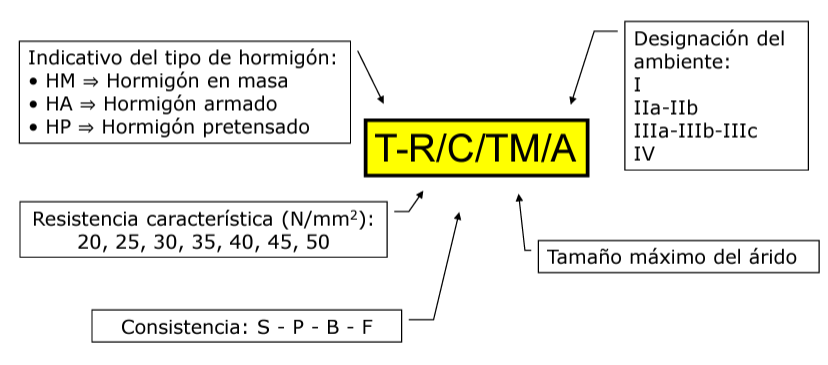
\includegraphics[width = 0.5 \textwidth]{Imagenes/Hormigon Especificacion.png}
\end{figure}

\section{Aceros estructurales.}
\subsection{Tipos.}
\begin{itemize}
    \item Perfiles laminados en caliente: Es el tipo más empleado en construcción. Se obtienen transformando el acero en bruto a alta temperaturra usando trenes de laminación. Se agrupan en series por la forma y características de su sección transversal (IPN IPE, HE, chapas, redondos, etc)
    \item Perfiles conformados en frío: Se fabrican mediante conformadoras de rodillo en frío a partir de chapas finas de acero. El conformado en frío les confiere unas características específicas en lo que se refiere a la sección y a la resistencia mecánica.
    \item Cables: Usados en puentes atirantados y colgantes y cubiertas de grandes luces. Se suele usar acero trefilado, que proporciona alta resistencia. Este acero se emplea también para el hormigón pretensado.
    \item Tornillos: Calidades de $4.6$ (tensión límite elástica $240\ MPa$) a $10.9$ (tensión elástica $900\ MPa$).
    \item Otros: Raíles, piezas para apoyos,...
\end{itemize}

\subsection{Características mecánicas.}
Ley de comportamiento de un acero de dureza natural.

\begin{figure}[H]
    \centering
    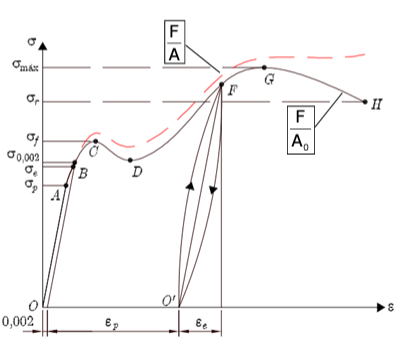
\includegraphics[width = 0.5 \textwidth]{Imagenes/Ley de comportamiento de un acero de dureza natural.png}
\end{figure}

Siendo:
\begin{itemize}
    \item $OA$: Zona elástica-lineal
    \item $AB$: Zona elástica
    \begin{itemize}
        \item $\sigma_p$: límite proporcionalidad
        \item $\sigma_e$: límite elástico (def. residual $2 \%$)
    \end{itemize}
    \item $BCDG$: Zona plástica
    \begin{itemize}
        \item $\sigma_f$: límite fluencia
        \item $\sigma_D$: límite inferior de fluencia
        \item $\sigma_{max}$: resistencia a la tracción
    \end{itemize}
    \item $O'F$: Rama descarga / recarga
    \begin{itemize}
        \item $\epsilon_p$: deformación plástica
        \item $\epsilon_e$: deformación elástica
    \end{itemize}
    \item $GH$: Estricción y rotura
    \begin{itemize}
        \item $\sigma_r$: tensión de rotura
    \end{itemize}
\end{itemize}

\begin{itemize}
    \item Límite elástico: Condiciona estados límites (alargamientos inaceptables de barras).
    \item Tensión de rotura: Condición estados límite (rotura de secciones).
    \item Endurecimiento: Permite el alargamiento de las barras.
    \item Alargamiento en rotura: Permite la redistribución de esfuerzos.
    \item Resistencia a rotura frágil: Condición previa a cualquier comprobación.
\end{itemize}

\subsubsection{Ductilidad}
Capacidad del acero de alcanzar grandes deformaciones sin llegar a la fractura.

Cuanto mayor sea el área encerrada por la zona plástica en el diagrama tensión-deformación, mayor será la ductilidad.

Los aceros dúctiles tienen mejor comportamiento a fratiga frente a cagas cíclicas.

Esta propiedad es muy importante en el proyecto sísmico de estructuras.

\subsection{Especificacion}

\begin{figure}[H]
    \centering
    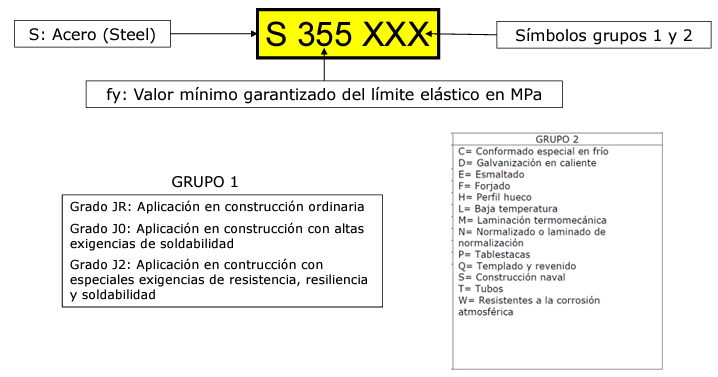
\includegraphics[width = 0.5 \textwidth]{Imagenes/Aceros Estructurales Especificacion.png}
\end{figure}

\section{Armaduras.}
\subsection{Tipos.}
\begin{itemize}
    \item Armaduras parivas: Es la armadura convencional utilizada en hormigón armado. Resisten las cargas pasivamente. Las resistencias habituales son $400$ ó $500\ MPa$. Tipologías
    \begin{itemize}
        \item Barras corrugadas rectas o rollos de acero
        \item Mallas electrosoldadas (forjados, muros, losas, zapatas, depósitos)
        \item Armaduras básicas electrosoldadas en celosía (prelosas, viguetas, ...)
    \end{itemize}
    \item Armaduras activas: Son las que se emplean en el hormmigón pretensado (tnedones o barras). Resisten las cargas activamente. Sólo se emplean aceros de alta resistencia ($> 1000\ MPa$).
\end{itemize}

\subsection{Especificación aceros empleados en armaduras pasivas}

\begin{figure}[H]
    \centering
    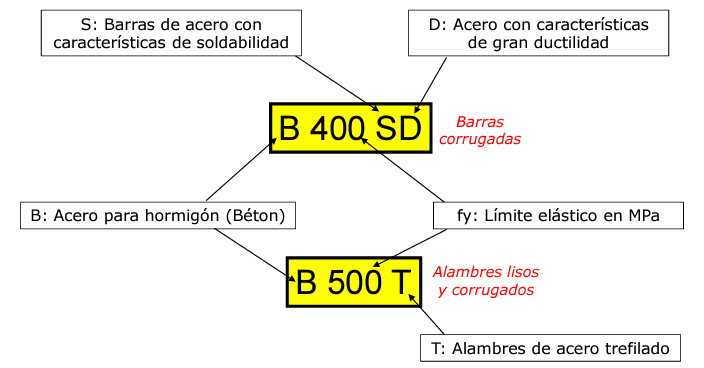
\includegraphics[width = 0.5 \textwidth]{Imagenes/Especificacion aceros empleados en armaduras pasivas.png}
\end{figure}

\subsection{Adherencia.}
La adherencia hormigón-acero es fundamental para que el hormigón armado pueda funcionar como material estructural. Mediante la adherencia se asegura el anclaje de las barras de acero y se controla la disuración del hormigón.

Los mecanismos de adherencia son de naturaleza físico-química (provocan la adhesión del acero con el hormigón a través de fuerzas capilares desarrolladas en la interfase) o mecánica (la penetración del cemento en las irregularidades de las barras provoca un efecto de rozamiento que favorece la adherencia y, además, en el caso de barras corrugadas, las corrugas hacen un efecto de cuña que aumenta la resistencia al deslizamiento).

% \section{Otros materiales de construcción.}

\section{Suelos}
\subsection{Generalidades.}
\begin{itemize}
    \item Rocas: masas minerales sin forma constante
    \item suelos: resultado alteración de las Rocas
    \item Materia orgánica
    \item Particularidades de suelos. El sulo presenta características muy distintas de otros materiales:
    \begin{itemize}
        \item No es posible su elección
        \item No se trata de un material homogéneo (aunque se intente asimilar).
        \item El contenido en agua tiene gran importancia en su comportamiento.
    \end{itemize}
\end{itemize}

\subsection{Clasificación.}
Arenas: alteración física de las rocas. Se caracterizan por no tener resistencia a tracción y sus propiedades dependen principalmente del tamaño de  partículas y su compacidad. Se clasifican mediante curvas granulométricas (tamizado de las muestras).

Arcillas: alteración química de las rocas. Son una mezcla de geles amorfos y partículas de especies mineralógicas generalmente con forma laminar. Sus propiedades dependen principalmente de la composición y humedad. Se clasifican mediante los límites de Atterberg (plasticidad frente a humedad).

\begin{itemize}
    \item Estructuras: 
    \begin{itemize}
        \item Floculadas (mayor índice huecos)
        \item Dispersas (ordenación de las láminas $\rightarrow$ menos resistencia corte). Se produce por una precompresión (preconsolidación) y es un proceso irreversible (memoria de las arcillas)
    \end{itemize}
    \item Plasticidad: El agua absorbida hace la función de lubricante
\end{itemize}

\subsection{Índices de fases.}
Suelo formado por la mezcla de tres fases (sólido, líquido y gas).
\begin{itemize}
    \item Suelos secos: huecos están llenos de aire.
    \item Suelos saturados: huecos están llenos de agua.
    \item Suelos parcialmente saturados: contienen aire y agua.
\end{itemize}

El agua en el suelo:
\begin{itemize}
    \item Agua Freática (acuíferos) - Nivel freático vs base rocosa
    \item Agua por encima del nivel freático:
    \begin{itemize}
        \item Agua higroscópica - fuerzas atracción
        \item Agua absorbida - tensión superficial
        \item Agua capilar - asciende de la capa freática
    \end{itemize}
\end{itemize}

\subsection{Propiedades elementales.}
\begin{itemize}
    \item Pesos específicos:
    \begin{itemize}
        \item Peso específico aparente: $\gamma = \frac{W_m}{V_m}$
        \item Peso específico seco: $\gamma_d = \frac{W_s}{V_m}$
        \item Pero específico saturado: $\gamma_{sat} = \frac{W_s + V_h \gamma_w}{V_m}$
        \item Peso específico sumergido: $\gamma' = \gamma_{sat} - \gamma_w$
        \item Peso específico fase sólida: $\gamma_s =\frac{W_s}{V_s} = G_s \gamma_w$; siendo $G_s$ la gravedad espcífica ($\approx 2.3$ a $2.8$)
    \end{itemize}
    \item Índices de fase:
    \begin{itemize}
        \item Índice de huecos: $e = \frac{V_a + V_w}{V_s}$
        \item Porosidad: $n = \frac{V_a + V_w}{V_m} = \frac{e}{1 + e }$
        \item Humedad: $w = \frac{W_w}{W_s} = \frac{W_m - W_s}{W_s}$
        \item Saturación: $S = \frac{V_w}{v_a + V_w}$
    \end{itemize}
\end{itemize}

\begin{figure}[H]
    \centering
    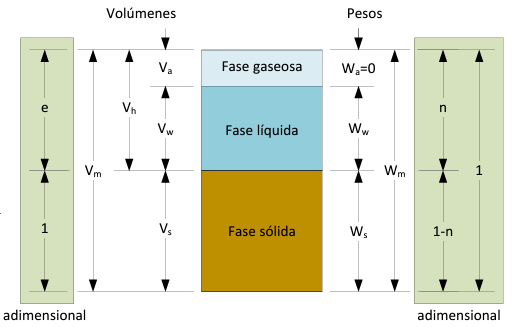
\includegraphics[width = 0.5 \textwidth]{Imagenes/Suelos Propiedades elementales.png}
\end{figure}

\subsection{Principio de Terzaghi o Principio de las tensiones efectivas.}
Representación del efcecto del agua en el suelo:
\begin{itemize}
    \item Equilibrio: tensiones totales
    \item Comportamiento: tensiones efectivas (no totales)
\end{itemize}
\[\sigma'_{ij} = \sigma_{ij} - u \cdot \delta_{ij}\]

Medio poroso. Analogía con una esponja sumerida en una bañera.
\begin{enumerate}
    \item Solo agua: no hay deformación.
    \item Agua y carga: hay deformación, los huecos comprimidos expulsan el agua.
\end{enumerate}

Reducción del nivel freático:

\begin{figure}[H]
    \centering
    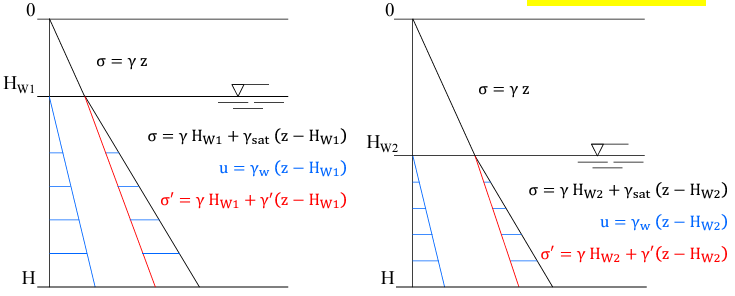
\includegraphics[width = 0.5 \textwidth]{Imagenes/Suelos Reduccion del nive freatico.png}
\end{figure}

\[(\gamma - \gamma') H_{w1} + \gamma' H \quad < \quad (\gamma - \gamma') H_{w2} + \gamma' H\]

\subsection{Modelo de comportamiento en Estado Límite de Servicio}
\subsubsection{Comprobación según CTE. Cálculo de Asientos}
\begin{itemize}
    \item Asiento s, definido como el descenso de cualquier punto de la cimentación de un edificio.
    \item Asiento diferencial, $\delta s$, definido como la diferencia de asiento entre dos puntos cualesquiera de la cimentación
    \item Distorsión angulas, $\beta$, definida como el asiento diferencial entre dos puntos dividido por la distancia que les separa.
    \item Inclinación, $\omega$, definida como el ángulo girado con respecto a la vertical según la línea media que define la posición deformada de la cimentación.
\end{itemize}

\begin{figure}[H]
    \centering
    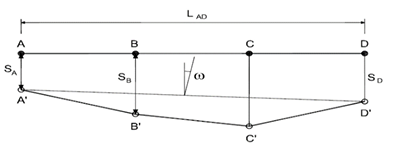
\includegraphics[width = 0.5 \textwidth]{Imagenes/Suelos Calculo de Asientos.png}
\end{figure}

\subsection{Consolidación}
\subsubsection{Importancia de la coexistencia de tres (dos) fases:}
\begin{itemize}
    \item Ley  de comportamiento(con tensiones efectivas) $\rightarrow$ Necesidad de ensayos de caracterización
    \item Permeabilidad $\rightarrow$ Resistencia al paso del agua por la estructura del suelo. Implica la variación temporal de las presiones neutras (drenaje del agua hasta alcanzar una nueva situación de equilibrio impedido por la resistencia que otroga la permeabilidad del suelo) y en consecuencia la aparición de un asiendo diferido en el tiempo $\rightarrow$ Consolidación
\end{itemize}

\subsection{Ley de comportamiento}
Ensayo edométrico: Se representa un terreno homogéneo con carga uniforma y difeerntes condiciones de drenaje.

Coeficiente de cambio volumétrico:
\[m_v = - \frac{d \epsilon_v}{d \sigma_a'}\]

